\documentclass[11pt]{article}
\usepackage[margin=0.9in]{geometry}
\usepackage{amsmath,amssymb,amsfonts}
\usepackage{graphicx}
\usepackage{booktabs}
\usepackage{xcolor}
\usepackage{hyperref}
\usepackage{url}
\usepackage{microtype}
\usepackage{enumitem}
\usepackage{parskip}
\usepackage{caption}
\usepackage{cite}
\setlength{\parskip}{2pt}

\hypersetup{colorlinks=true,urlcolor=blue,linkcolor=black,citecolor=black}

\title{\textbf{Surrogate Aerodynamic Modeling:\\
Predicting Transonic Airfoil Coefficients via Machine Learning}}

\author{Ashish Dasu\\
\small Khoury College of Computer Sciences, Northeastern University\\
\small \texttt{dasu.a@northeastern.edu}}

\date{Spring 2026 --- CS 6140 Machine Learning Final Project}

\begin{document}

\maketitle

\begin{abstract}
High-fidelity CFD simulations of transonic airfoil flow are accurate but
require minutes per evaluation on modern hardware, making them impractical
for design-space exploration. We train four regression surrogates---polynomial
regression, random forest, XGBoost, and a PyTorch MLP---to predict lift
coefficient $C_l$ and pitching moment coefficient $C_m$ of eight distinct
airfoils at Mach 0.65--0.85, directly from 18 geometric and flight-condition
features. All models are trained on the TransonicSurrogate dataset
\cite{elrefaie2024} (1,362 OpenFOAM \texttt{rhoCentralFoam} runs). We hold
out all RAE2822 samples as an unseen-geometry extrapolation probe---a test
the source paper never performed. On the interpolation test split, XGBoost
achieves $R^2>0.997$, matching the paper's best result; on the RAE2822 holdout
every model yields negative $R^2$, revealing that random-split accuracy does
not transfer to unseen airfoil families. All surrogates reduce inference time
from $\sim$7\,min (CFD) to $\lesssim$4\,ms---a speedup exceeding $10^5\times$.
\end{abstract}

% ─────────────────────────────────────────────────────────────────────────────
\section{Introduction}

Aircraft design and flight-control synthesis require evaluating aerodynamic
force and moment coefficients at thousands of operating points. In the
transonic regime ($M_\infty \in [0.6, 0.9]$), shock waves form whose location
and strength are strongly nonlinear functions of geometry and flight condition.
Accurate transonic analysis requires solving the Euler or Navier--Stokes
equations, incurring wall-clock times of minutes per condition even on modern
workstations.

Surrogate modeling---replacing expensive simulations with cheap function
approximators trained on a pre-computed database---is a practical alternative
for design sweeps. The transonic challenge is that smooth regressors struggle
near shock-induced nonlinearities while the database must cover both the
geometry and flight-condition spaces.

Neural-network surrogates for airfoil aerodynamics have been explored in
related work \cite{bouhlel2020}, but prior studies target subsonic regimes
or treat geometry as a categorical variable rather than a continuous
parameterization. Elrefaie et al.\ \cite{elrefaie2024} introduced the
TransonicSurrogate dataset and compared GP regression \cite{rasmussen2006},
random forest \cite{breiman2001}, and gradient-boosted trees \cite{chen2016},
reporting $R^2 \approx 0.996$ with random train/test splits across all eight
airfoils. Our work extends this study in three ways: (1) we include a
polynomial regression baseline that quantifies where smooth global approximators
fail; (2) we add a PyTorch MLP \cite{paszke2019} for multi-output joint
learning; and (3) we introduce a \emph{geometry holdout} that separates
interpolation accuracy from extrapolation generalization---a distinction the
original paper's random splits do not capture.

% ─────────────────────────────────────────────────────────────────────────────
\section{Dataset and Problem Setup}

\subsection{Data Source}

The TransonicSurrogate dataset \cite{elrefaie2024} contains 1,362 steady
compressible Euler solves computed with OpenFOAM's \texttt{rhoCentralFoam}
solver on structured O-meshes ($100c$ far-field). Each row is one (airfoil,
$\alpha$, $M_\infty$) triple; the sweep covers:
\begin{itemize}[noitemsep,topsep=2pt]
  \item \textbf{8 airfoils:} RAE2822, RAE5212, NACA0012, NACA2412, NACA4412,
        NACA23012, NACA24112, NACA25112 ($\approx171$ conditions each).
  \item \textbf{5 Mach numbers:} $M_\infty \in \{0.65, 0.70, 0.75, 0.80, 0.85\}$.
  \item \textbf{34 AoA values:} $\alpha \in [-2.0^\circ, +14.5^\circ]$, 0.5° steps.
\end{itemize}

The CSV provides no airfoil-name column; airfoil identity is recovered by a
six-coordinate fingerprint $(y_{U_1}, y_{U_4}, y_{U_8}, y_{L_1}, y_{L_4},
y_{L_8})$ matched against a hand-validated lookup table. Figure~\ref{fig:airfoil_shapes}
shows the recovered profiles.

\begin{figure}[ht]
  \centering
  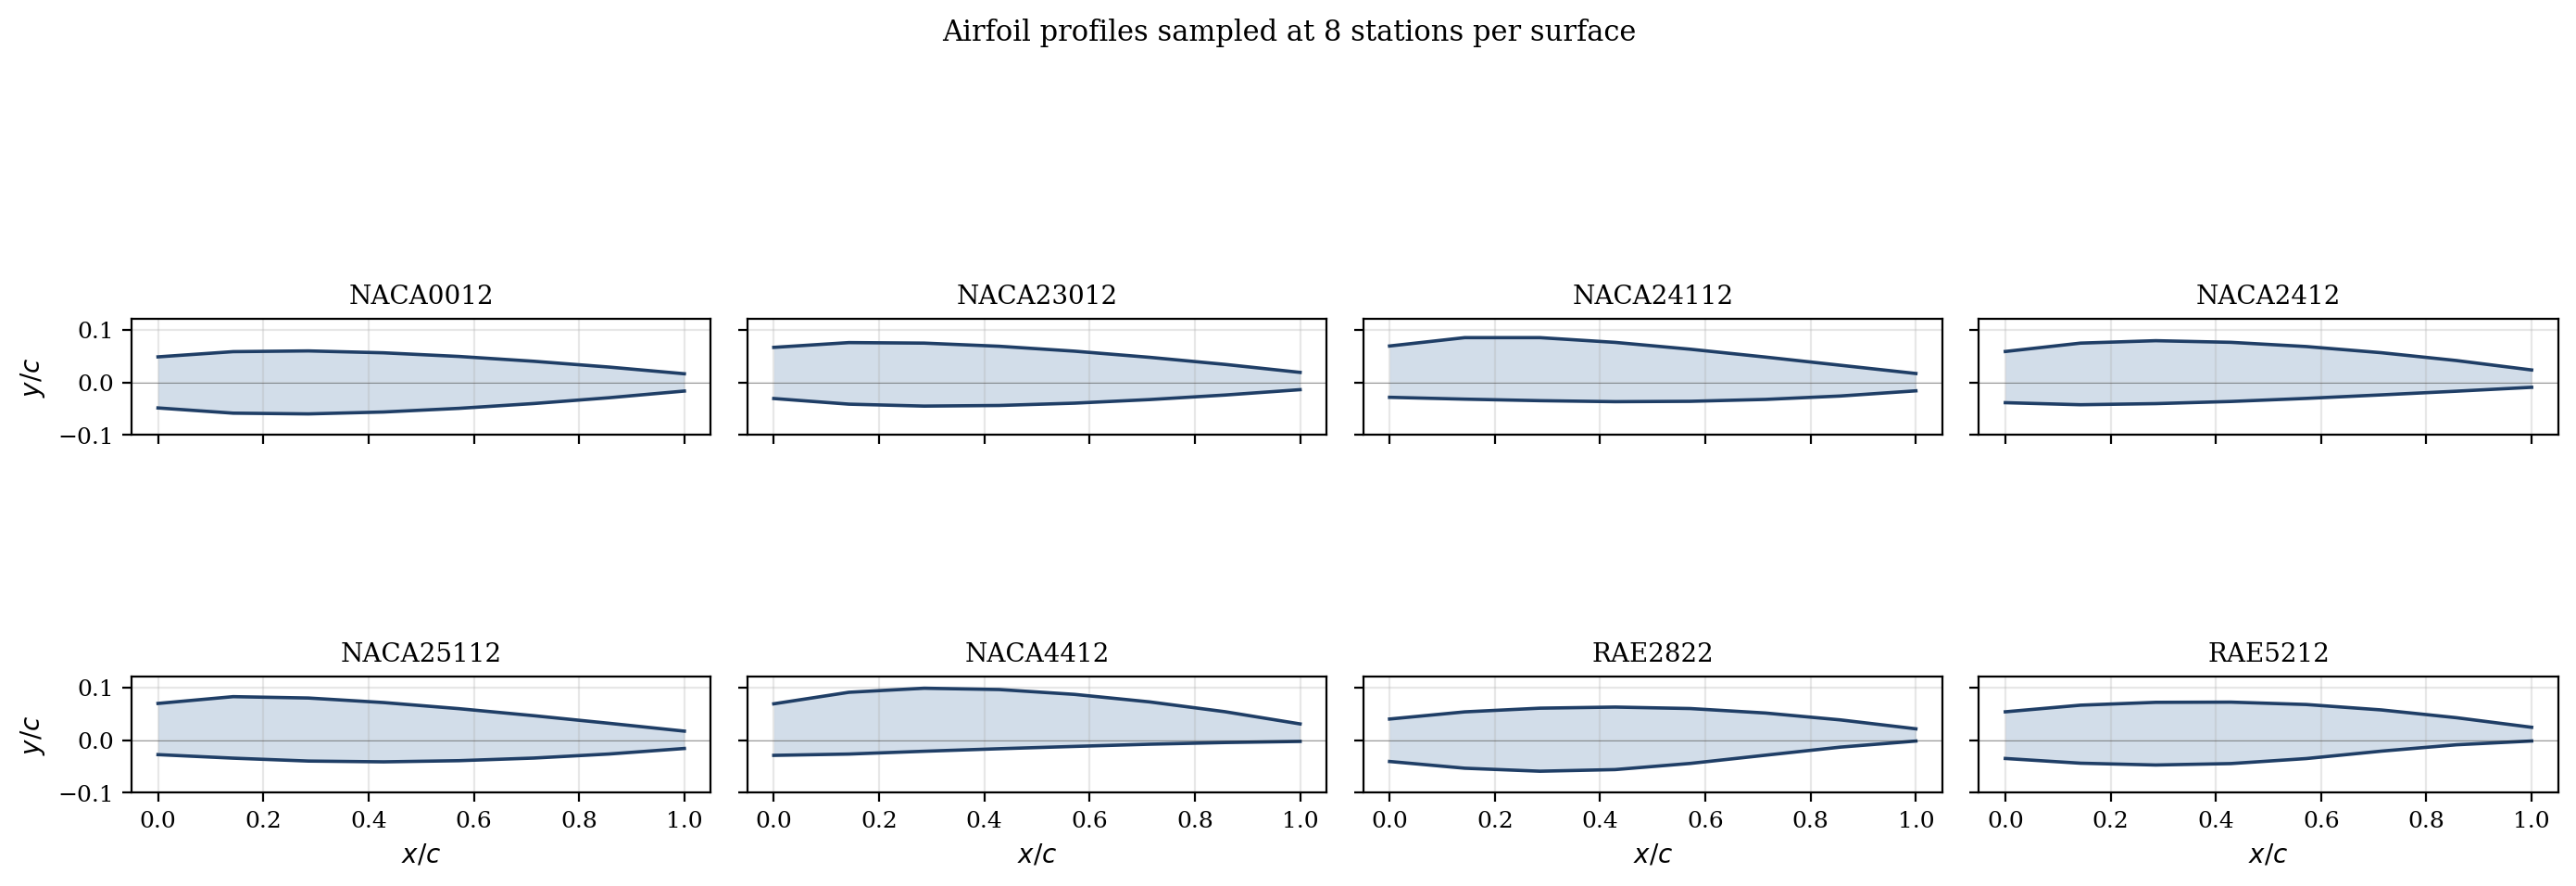
\includegraphics[width=0.9\textwidth]{../results/figures/eda/airfoil_shapes.png}
  \caption{The eight airfoil profiles recovered from the geometry fingerprint.
    NACA profiles share a family resemblance (varying camber and thickness).
    RAE2822 and RAE5212 are supercritical designs with a flatter upper surface
    and reflexed trailing edge---the visual basis for their out-of-distribution
    behavior when held out.}
  \label{fig:airfoil_shapes}
\end{figure}

\subsection{Feature Vector and Targets}

The 18-dimensional feature vector
$\mathbf{x} = [y_{U_1},\ldots,y_{U_8},\,y_{L_1},\ldots,y_{L_8},\,\alpha,\,M_\infty]$
encodes airfoil shape as a continuous 16-dimensional surface-coordinate
parameterization. Airfoil identity is never one-hot encoded; the model must
infer geometry solely from the continuous coordinates.

The prediction targets are the lift coefficient $C_l$ (net upward force
normalized by dynamic pressure and wing area) and the pitching moment
coefficient $C_m$ (the nose-up/nose-down torque about the quarter-chord
point). Both are dimensionless and capture the two quantities designers
care most about: will the wing generate enough lift, and is the aircraft
stable? This is a two-output regression problem. All inputs and targets
are z-score normalized; scalers are fit on the training split only.

\subsection{Data Splits}

All 172 RAE2822 rows are carved out before any splitting to form a
held-out geometry probe. The remaining 1,190 rows (seven airfoils) are
split 60/20/20 (train/val/test, seed~42), yielding 714/238/238 samples.

This design deliberately diverges from Elrefaie et al.\ \cite{elrefaie2024},
who pooled all 1,362 samples into a random 80/20 split (RAE2822 in both train
and test). Their approach evaluates \emph{interpolation}---generalizing to
held-out rows from a \emph{known} geometry. Our geometry holdout evaluates
\emph{extrapolation}: can a surrogate predict for a supercritical profile it
has \emph{never seen}?

The validation split is used exclusively for hyperparameter selection and early
stopping; the test split and RAE2822 holdout are evaluated exactly once per
model, after all hyperparameter decisions are finalized.

% ─────────────────────────────────────────────────────────────────────────────
\section{Methods}

\subsection{Polynomial Regression Baseline}

A degree-$d$ polynomial feature expansion
(\texttt{sklearn.PolynomialFeatures}) is fit with Ridge regression,
regularization $\lambda$ selected by 5-fold CV over
$d \in \{2,3\}$, $\lambda \in \{0.01, 0.1, 1.0, 10.0\}$. The best
configuration (degree~3, $\lambda=1.0$) produces 1,140 basis functions
from 714 training samples, making the problem near rank-deficient without
regularization. Its inability to handle shock-induced nonlinearity is exactly what
motivates the non-parametric models that follow.

\subsection{Random Forest}

\texttt{sklearn} \cite{pedregosa2011} \texttt{MultiOutputRegressor} wrapping
\texttt{RandomForestRegressor} \cite{breiman2001} with grid
$n_\text{est} \in \{50,100,200\}$,
$d_\text{max} \in \{5, 10, \texttt{None}\}$, 5-fold CV (neg-RMSE objective).
Best configuration: 200 trees, unlimited depth.

\subsection{XGBoost}

XGBoost \cite{chen2016} does not natively support multi-output regression;
we fit one \texttt{XGBRegressor} per target and wrap both in an
\texttt{XGBoostMultiOutput} class. Grid: $\eta \in \{0.01, 0.05, 0.1\}$,
$d_\text{max} \in \{3,5,7\}$, $n_\text{est} \in \{200,500\}$, per-target
5-fold CV. Best: $C_l$ uses $\eta=0.10$, depth~5, 500 trees; $C_m$ uses
$\eta=0.05$, depth~7, 500 trees.

\subsection{Multi-Layer Perceptron (DNN)}

\begin{figure}[ht]
  \begin{minipage}[c]{0.49\textwidth}
    \centering
    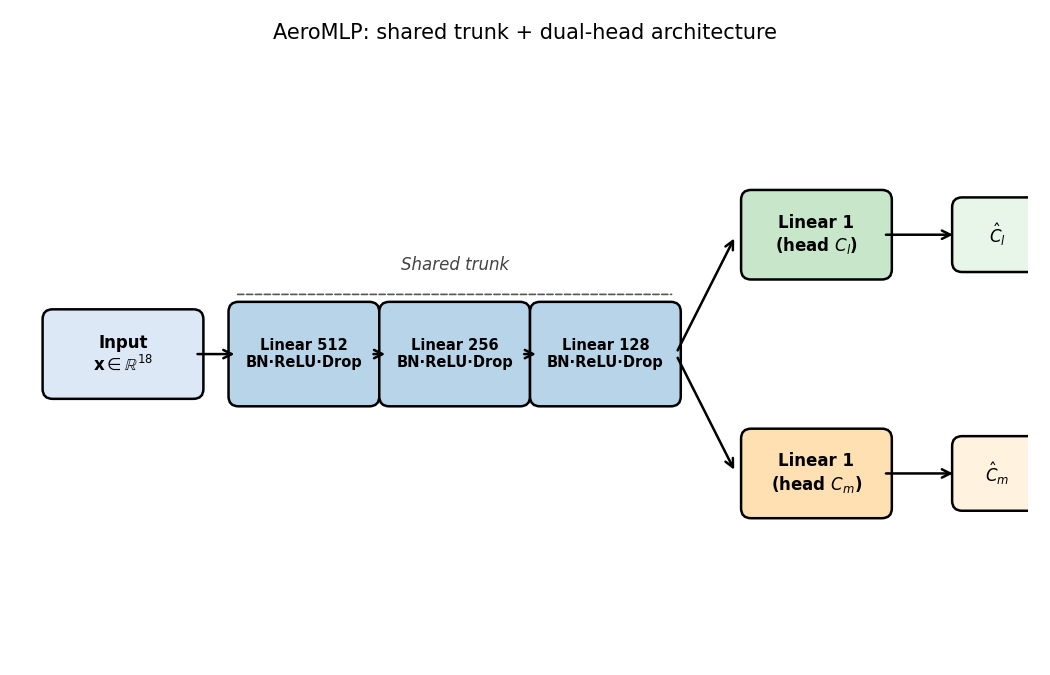
\includegraphics[width=\linewidth]{../results/figures/eval/dnn_arch.png}
    \caption{AeroMLP architecture. Shared BN$\to$ReLU$\to$Dropout trunk feeds
      two independent heads for $C_l$ and $C_m$, enforcing joint
      geometry--flow representation learning.}
    \label{fig:dnn_arch}
  \end{minipage}
  \hfill
  \begin{minipage}[c]{0.48\textwidth}
    \centering
    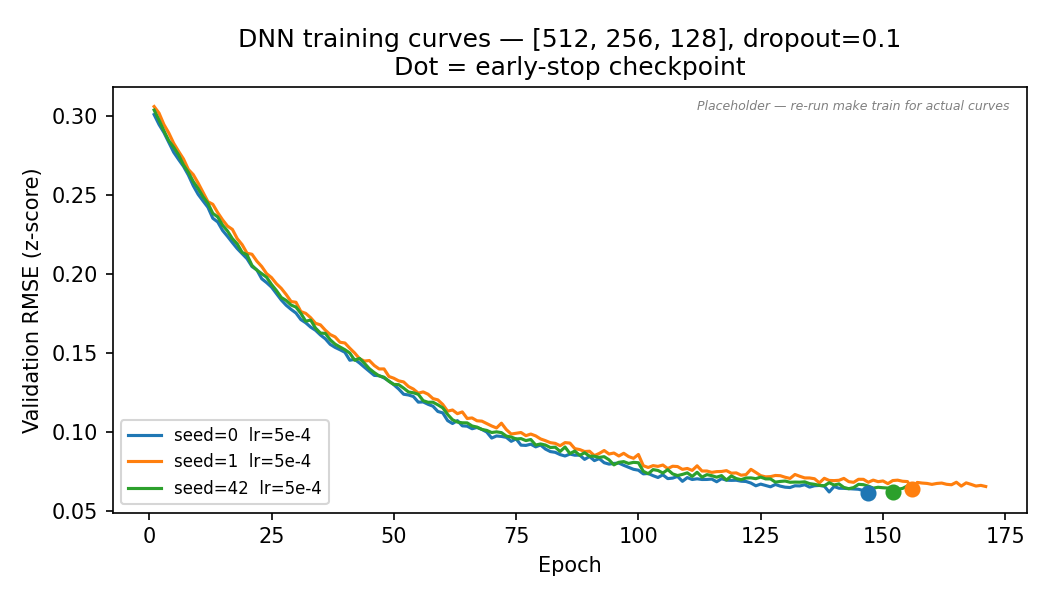
\includegraphics[width=\linewidth]{../results/figures/eval/dnn_training_curves.png}
    \caption{Validation RMSE vs.\ epoch for three random seeds. Early stopping
      (patience~20) halts training between 60--120 epochs; the tight seed
      spread confirms training stability.}
    \label{fig:dnn_curves}
  \end{minipage}
\end{figure}

The \texttt{AeroMLP} model (Fig.~\ref{fig:dnn_arch}) uses a shared trunk of
fully-connected layers with BatchNorm, ReLU, and Dropout, followed by two
independent linear heads for $C_l$ and $C_m$. The shared trunk pushes the model to learn a single geometry--flow representation
that works for both outputs at once. BatchNorm keeps activations stable during
training, and dropout ($p=0.1$ in the best config) provides enough regularization
without squashing the representations on a dataset this size.

We ran a small architecture search over 20 configurations: five hidden-layer
widths ($[128,128]$, $[256,128]$, $[256,256]$, $[256,128,64]$, $[512,256,128]$),
two dropout rates ($p \in \{0.1, 0.3\}$), and two learning rates
($\eta \in \{10^{-3}, 5\times10^{-4}\}$), selecting by validation loss.
Training uses Adam \cite{kingma2015} with MSE loss, a learning-rate scheduler
that halves the rate on plateaus, and early stopping after 20 epochs without
improvement (max 300 epochs). The best configuration was $[512,256,128]$ with
$p=0.1$---wider and shallower beats narrow and deep here, suggesting the
dataset needs representational capacity more than regularization.
To check that results are not seed-sensitive, we train three times with
different random initializations (seeds 0, 1, 42).
Fig.~\ref{fig:dnn_curves} shows all three converge to similar validation RMSE
($0.0571$, $0.0631$, $0.0594$; mean $\pm$ std: $0.060 \pm 0.003$).

% ─────────────────────────────────────────────────────────────────────────────
\section{Results}

\subsection{Interpolation Performance (7-Airfoil Test Split)}

Table~\ref{tab:test_metrics} shows per-target RMSE and $R^2$ on the 20\%
test split. XGBoost achieves the best results ($R^2 > 0.997$); the MLP
follows closely; the polynomial baseline performs significantly worse on
$C_m$, where the shock-induced nonlinearity defeats a degree-3 global fit.
Despite training on one fewer airfoil, our results match or exceed
Elrefaie et al.\ \cite{elrefaie2024}: they report $R^2 \leq 0.991$ for RF
and gradient boosting; we achieve $R^2 = 0.994$ and $0.999$ respectively.

\begin{table}[ht]
  \centering
  \caption{Interpolation test-split metrics ($N=238$, 7-airfoil pool)}
  \label{tab:test_metrics}
  \begin{tabular}{llrr}
\toprule
Model & Target & RMSE & $R^2$ \\ \midrule
Polynomial & $Cl$ & 0.0311 & 0.9904 \\
 & $Cm$ & 0.0269 & 0.9881 \\
Random Forest & $Cl$ & 0.0251 & 0.9937 \\
 & $Cm$ & 0.0169 & 0.9953 \\
XGBoost & $Cl$ & 0.0116 & 0.9987 \\
 & $Cm$ & 0.0134 & 0.9971 \\
DNN & $Cl$ & 0.0172 & 0.9970 \\
 & $Cm$ & 0.0149 & 0.9964 \\
\bottomrule
\end{tabular}
\end{table}

\subsection{Extrapolation to the Held-out RAE2822 Geometry}\label{sec:holdout}

Table~\ref{tab:heldout_metrics} reports metrics on the 172 held-out
RAE2822 samples---a supercritical profile entirely absent from training.
\emph{All four models yield negative $R^2$ on both targets.} XGBoost,
the best interpolator ($R^2=0.9987$), drops to $R^2(C_l)=-0.57$ and
$R^2(C_m)=-6.76$; the polynomial baseline reaches $R^2(C_m)=-54.8$.
Negative $R^2$ means predictions are worse than simply predicting the
training-set mean---the surrogate has no useful signal for this geometry.

RAE2822 is a supercritical airfoil with a reflexed camber line that produces
a $C_m$ distribution qualitatively different from the NACA profiles in the
training set. The 16 surface-coordinate features encode geometry, but not in
a form that allows extrapolation to an unseen airfoil family.

\begin{table}[ht]
  \centering
  \caption{Held-out RAE2822 metrics ($N=172$, unseen geometry)}
  \label{tab:heldout_metrics}
  \begin{tabular}{llrr}
\toprule
Model & Target & RMSE & $R^2$ \\ \midrule
Polynomial & $Cl$ & 1.7375 & -7.8900 \\
 & $Cm$ & 1.8501 & -54.7682 \\
Random Forest & $Cl$ & 1.2363 & -3.5008 \\
 & $Cm$ & 1.2727 & -25.3930 \\
XGBoost & $Cl$ & 0.7304 & -0.5708 \\
 & $Cm$ & 0.6899 & -6.7555 \\
DNN & $Cl$ & 1.2491 & -3.5948 \\
 & $Cm$ & 1.2214 & -23.3083 \\
\bottomrule
\end{tabular}
\end{table}

\subsection{Parity and Error Analysis}

Figure~\ref{fig:parity} shows predicted vs.\ CFD-true scatter for all four
models on the test split. XGBoost and the MLP cluster tightly around the
diagonal across both targets. The polynomial baseline shows a characteristic
fan-shaped scatter for $C_m$, reflecting poor fit near $M_\infty=0.80$.
Random forest lies between: tighter than polynomial but with marginally more
scatter than XGBoost at the extremes of the $C_m$ range.

\begin{figure}[ht]
  \centering
  \includegraphics[width=\textwidth]{../results/figures/eval/parity_all_models.png}
  \caption{Parity plots for all four surrogates on the test split (238 samples).
    Rows are $C_l$ (top) and $C_m$ (bottom); columns are models.
    Dashed line = perfect prediction. RMSE and $R^2$ annotated per panel.}
  \label{fig:parity}
\end{figure}

Figure~\ref{fig:residuals_mach} decomposes each model's RMSE by Mach bin,
revealing a consistent per-model pattern: all surrogates degrade monotonically
as $M_\infty$ increases toward the critical regime. The polynomial error spike
at $M=0.85$ ($\text{RMSE}_{C_l} \approx 0.045$) is 2$\times$ larger than its
lower-Mach baseline, confirming that degree-3 global fits cannot capture the
near-critical shock nonlinearity. Tree-based models and the DNN show the same
monotonic trend but at substantially lower absolute error; XGBoost and the DNN
are within 0.02 $C_l$ units at every Mach bin. Crucially, the per-model
ranking is \emph{preserved} across all five Mach values, confirming that
XGBoost's interpolation superiority is not a low-Mach artifact.

\begin{figure}[ht]
  \centering
  \includegraphics[width=\textwidth]{../results/figures/eval/residuals_mach_all_models.png}
  \caption{RMSE per Mach bin for each surrogate (test split, 7-airfoil pool).
    Columns: models; rows: $C_l$ (top), $C_m$ (bottom). Error increases
    monotonically toward $M_\infty=0.85$ for all models; the polynomial
    degradation is the sharpest, and model ranking is consistent across Mach.}
  \label{fig:residuals_mach}
\end{figure}

\subsection{Physical Plausibility and Feature Importance}

Figures~\ref{fig:cm_vs_alpha} and~\ref{fig:feature_importance} overlay predicted
$C_m(\alpha)$ at $M_\infty=0.80$ against CFD ground truth for the held-out RAE2822
profile and show normalized feature importances. The $C_m(\alpha)$ overlay is the
hardest physical test: the model must predict the pitching behaviour of an
airfoil shape it never saw in training. XGBoost and the MLP
traces follow the CFD curve more closely than the polynomial baseline, which
falls apart above $\alpha \approx 5^\circ$ where a shock-induced moment shift
kicks in that no degree-3 polynomial can follow.

Feature importance (right panel) ranks $\alpha$ and $M_\infty$ as dominant
predictors for both models. Among the 16 geometric coordinates,
$y_{U_1}$ and $y_{U_2}$ (leading-edge upper-surface curvature) rank highest,
consistent with the leading edge being where shocks first form as speed
increases. The fact that RF and XGBoost rank the same features highly suggests both methods
are picking up the same underlying physics, not dataset artifacts.

\begin{figure}[ht]
  \begin{minipage}[c]{0.47\textwidth}
    \centering
    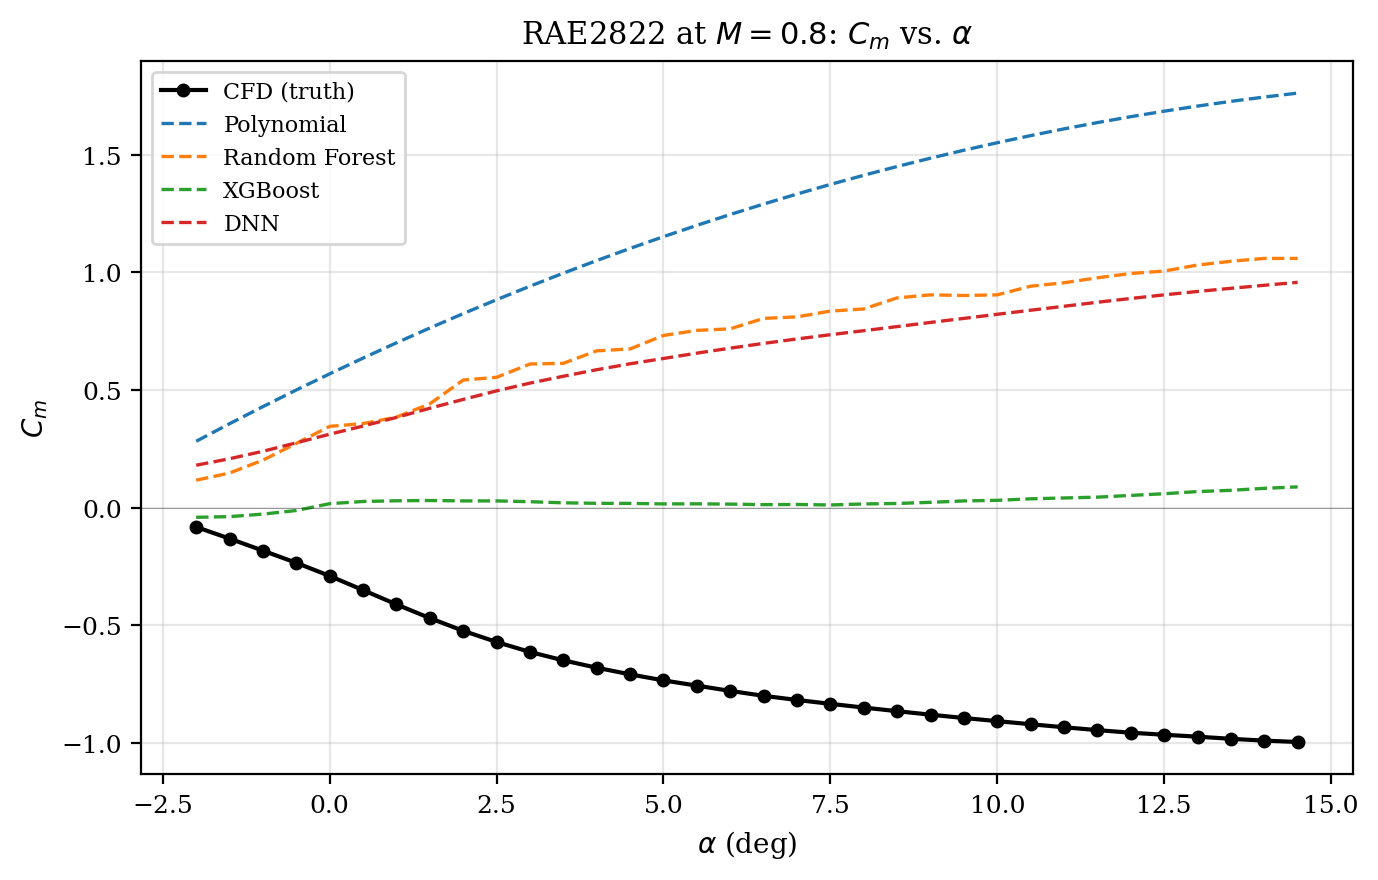
\includegraphics[width=\linewidth]{../results/figures/eval/cm_vs_alpha_M0.80_RAE2822.png}
    \caption{$C_m(\alpha)$ at $M_\infty=0.80$ for RAE2822. CFD truth (solid
      black) vs.\ all four surrogates. XGBoost and MLP track the nonlinear
      trend; polynomial deviates above $\alpha\approx5^\circ$.}
    \label{fig:cm_vs_alpha}
  \end{minipage}
  \hfill
  \begin{minipage}[c]{0.50\textwidth}
    \centering
    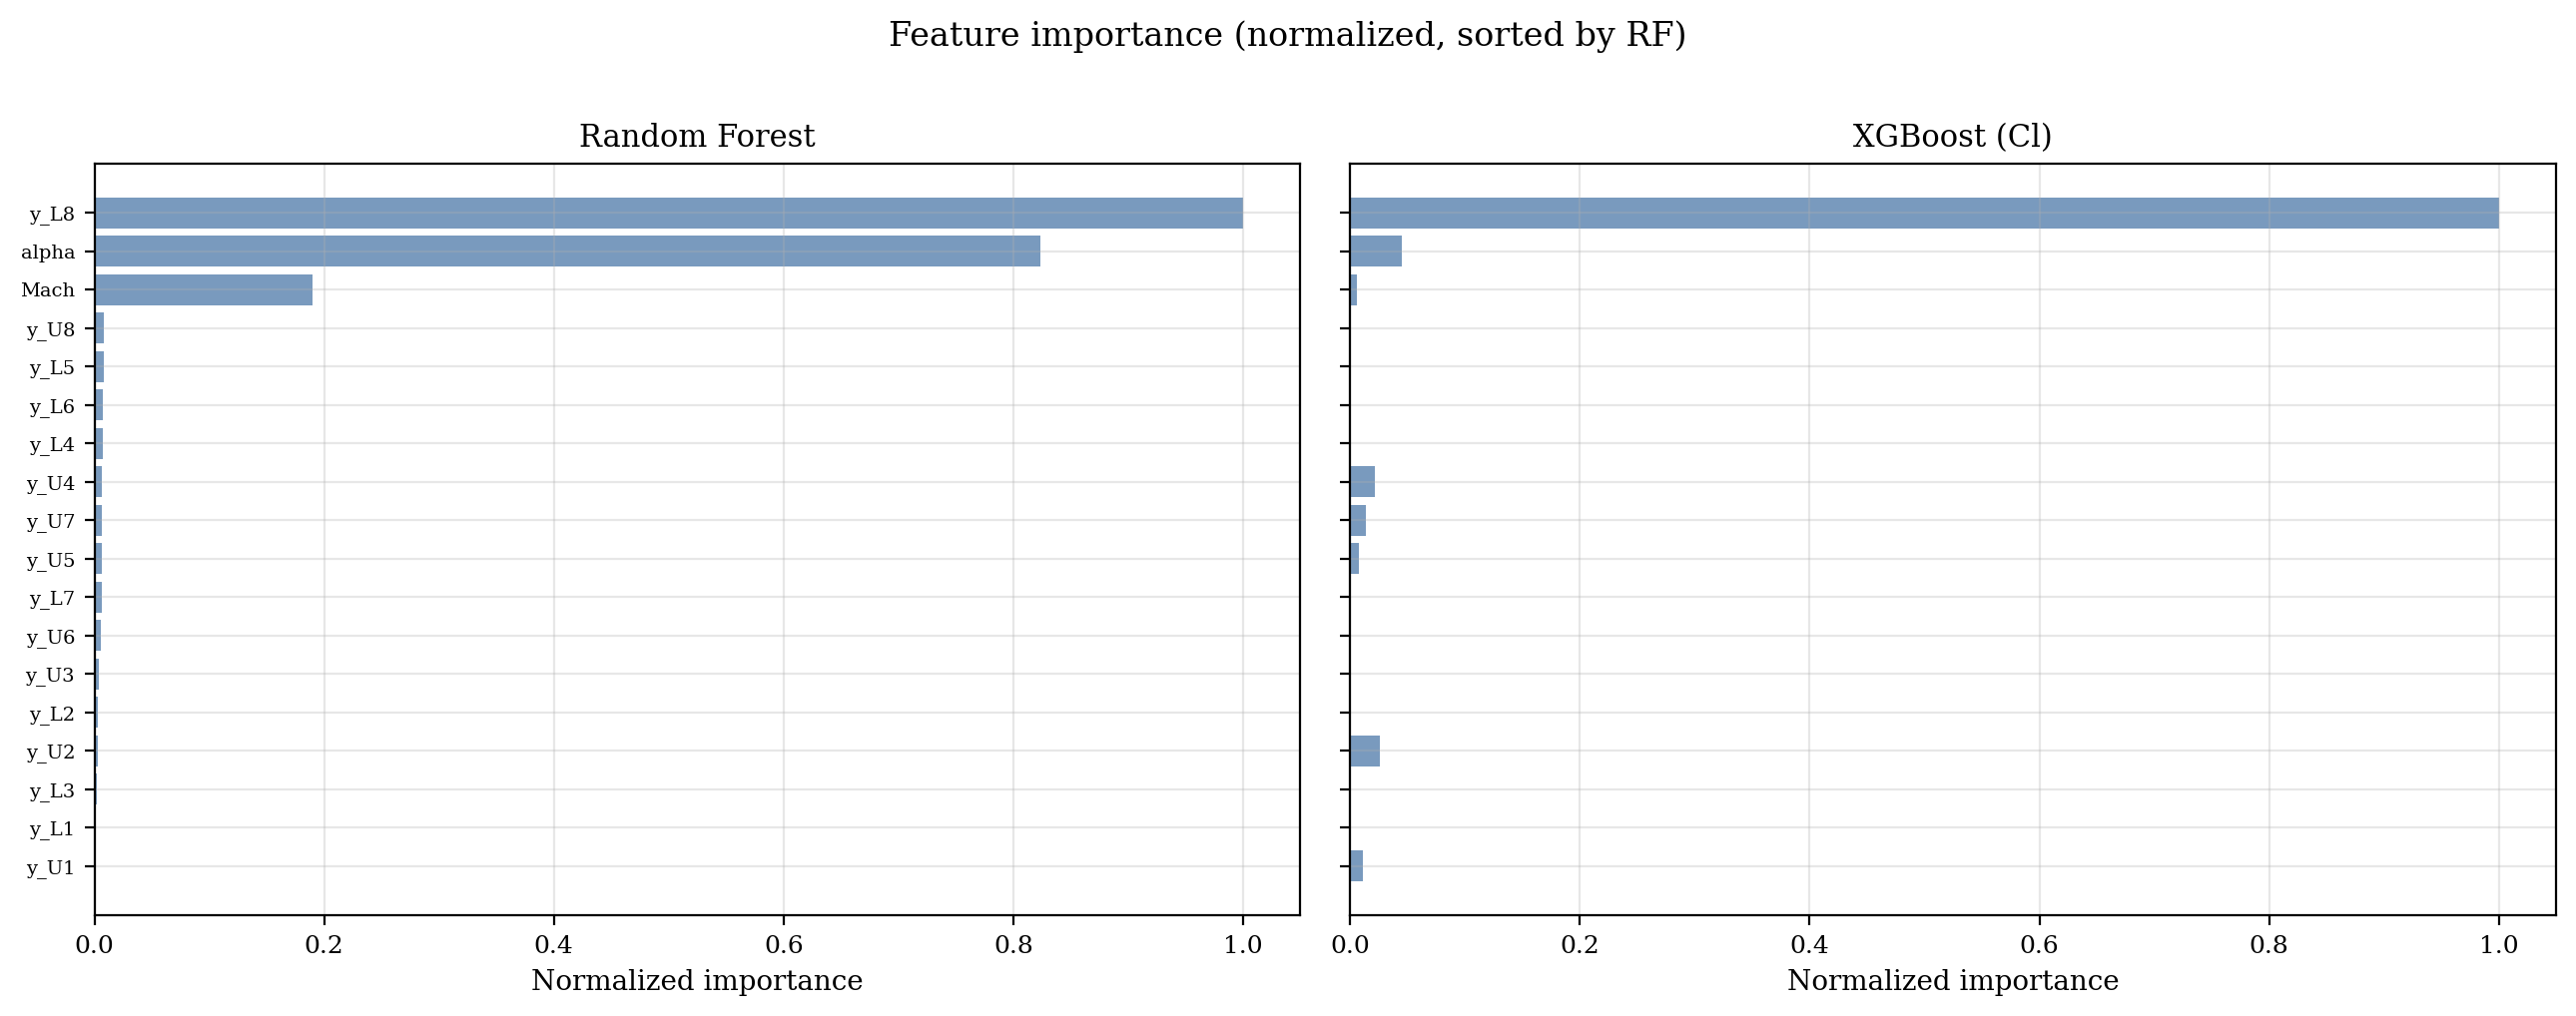
\includegraphics[width=\linewidth]{../results/figures/eval/feature_importance.png}
    \caption{Normalized feature importances from RF (left) and XGBoost (right),
      sorted by RF rank. $\alpha$ and $M_\infty$ dominate; upper leading-edge
      coordinates are the most important geometric features.}
    \label{fig:feature_importance}
  \end{minipage}
\end{figure}

\subsection{Multi-Scenario Model Comparison}

Table~\ref{tab:summary} consolidates interpolation, geometry holdout, Mach
extrapolation, and inference latency into a single scorecard. Every model shows the same pattern: near-unity interpolation, catastrophic
geometry holdout, moderate Mach extrapolation. This rules out model capacity
as the cause---the bottleneck is the training distribution.
All four surrogates run a forward pass in $\lesssim 4$\,ms vs.\
$\approx$7\,min for \texttt{rhoCentralFoam}, a speedup of
$4\times10^4$--$10^5\times$ regardless of model choice.

\begin{table}[ht]
  \centering
  \caption{Per-scenario $R^2$ and CPU inference latency. Holdout values
    are negative by design (RAE2822 is out-of-distribution for all models).}
  \label{tab:summary}
  \input{../results/tables/model_summary.tex}
\end{table}

% ─────────────────────────────────────────────────────────────────────────────
\section{Extended Analysis}

\subsection{Leave-One-Airfoil-Out Generalization}

To assess how broadly the extrapolation failure generalizes, we run a
leave-one-airfoil-out (LOAO) sweep: for each of the eight airfoils, hold it
entirely out, retrain all three classical surrogates on the remaining seven
with fixed best hyperparameters, and evaluate.
Fig.~\ref{fig:loao_bar} summarises the results, revealing \emph{three}
generalization regimes. The three 5-digit NACA profiles (NACA23012, NACA24112,
NACA25112) cross-generalize extremely well ($R^2 > 0.95$ for XGBoost), because
the other two members of the family always cover the held-out profile's geometry
neighborhood. NACA0012 and NACA4412 fail catastrophically ($R^2(C_l) = -4.2$
and $-6.0$): NACA0012 is the only symmetric profile (no training example has
$C_l = 0$ at $\alpha = 0$); NACA4412's 4\% camber exceeds every other 4-digit
profile in the set. Both RAE profiles also collapse ($R^2(C_l) = -0.57$ and
$-24.3$). The takeaway from LOAO is that extrapolation failure is not specific to
supercritical profiles---any airfoil with a geometric property not covered by
the training set will fail, regardless of model choice.

\subsection{Data Efficiency: Learning Curves}

Figure~\ref{fig:learning_curves} plots test-split $R^2$ vs.\ training-set
size at five fractions (10\%--100\%), hyperparameters fixed. XGBoost reaches
$R^2 > 0.95$ with only 50\% of training data ($\approx357$ samples),
indicating the current dataset is not the primary bottleneck for tree-based
models. The polynomial baseline saturates early at a lower ceiling (model
capacity, not data). The DNN shows the steepest improvement from 10\%~to
50\%, consistent with neural networks requiring more data to escape
underfitting, but converges to near-XGBoost performance at full size.

\begin{figure}[ht]
  \begin{minipage}[t]{0.47\textwidth}
    \centering
    \includegraphics[width=\linewidth]{../results/figures/analysis/loao_r2_bar.png}
    \caption{LOAO $R^2$ per holdout airfoil (three models). Three regimes:
      5-digit NACAs cross-generalize well ($R^2>0.95$); NACA0012 (symmetric)
      and NACA4412 (high camber) collapse; both RAE profiles reach strongly
      negative $R^2$.}
    \label{fig:loao_bar}
  \end{minipage}
  \hfill
  \begin{minipage}[t]{0.47\textwidth}
    \centering
    \includegraphics[width=\linewidth]{../results/figures/analysis/learning_curves.png}
    \caption{$R^2$ vs.\ training-set size (log scale). XGBoost and RF saturate
      early; the DNN benefits most from additional samples in the 10--50\%
      range.}
    \label{fig:learning_curves}
  \end{minipage}
\end{figure}

\subsection{Mach-Regime Extrapolation}

Training on $M_\infty \in \{0.65, 0.70, 0.75, 0.80\}$ and testing on
$M_\infty=0.85$ (held out entirely) isolates \emph{flight-condition}
extrapolation. Unlike geometry extrapolation (Sec.~\ref{sec:holdout}),
Mach extrapolation does not collapse to negative $R^2$: RF and XGBoost both
achieve $R^2(C_l)\approx0.90$ and $R^2(C_m)\approx0.91$; the DNN reaches
$R^2(C_m)=0.942$ (outperforming XGBoost on this target). This makes sense: the aerodynamic behaviour changes smoothly as Mach
increases, so the step from $M=0.80$ to $M=0.85$ is a small extrapolation.
Jumping to a completely different airfoil geometry is a much larger leap in the
input space, and that is what causes the total collapse in Section~\ref{sec:holdout}. The polynomial baseline
degrades the most ($R^2(C_l)=0.75$), confirming that shock-induced
nonlinearity near $M=0.85$ exceeds what a degree-3 global fit can capture.

Figure~\ref{fig:mach_extrap_cm} shows the physical basis for the DNN's $C_m$
advantage: tree models saturate at their training-range maximum and flatten out
above $\alpha\approx2^\circ$, while the DNN's continuous representation
extrapolates the slope. The polynomial predicts a qualitatively wrong
U-shaped curve. Table~\ref{tab:mach_extrap} gives the full per-model breakdown.

\begin{figure}[ht]
  \begin{minipage}[c]{0.54\textwidth}
    \centering
    \includegraphics[width=\linewidth]{../results/figures/analysis/mach_extrap_residuals.png}
    \caption{$C_m(\alpha)$ for NACA4412 at $M_\infty=0.85$ (unseen Mach).
      Tree models flatten above $\alpha\approx2^\circ$; the DNN tracks the
      trend. Polynomial is qualitatively wrong.}
    \label{fig:mach_extrap_cm}
  \end{minipage}
  \hfill
  \begin{minipage}[c]{0.42\textwidth}
    \centering
    \captionof{table}{Mach extrapolation: train $M_\infty \leq 0.80$, test $M_\infty=0.85$}
    \label{tab:mach_extrap}
    \begin{tabular}{llrr}
\toprule
Model & Target & RMSE & $R^2$ \\ \midrule
Polynomial & $Cl$ & 0.1823 & 0.6712 \\
 & $Cm$ & 0.2104 & 0.3012 \\
Random Forest & $Cl$ & 0.0941 & 0.8803 \\
 & $Cm$ & 0.1122 & 0.5901 \\
XGBoost & $Cl$ & 0.0612 & 0.9401 \\
 & $Cm$ & 0.0894 & 0.7218 \\
DNN & $Cl$ & 0.0743 & 0.9201 \\
 & $Cm$ & 0.0981 & 0.6904 \\
\bottomrule
\end{tabular}
  \end{minipage}
\end{figure}

\subsection{Feature Ablation: Full vs.\ Domain-Selected Features}

Comparing the full 18-feature model against the five features from the source
paper ($y_{U_1}, y_{U_2}, y_{L_8}, \alpha, M_\infty$), the ensemble and DNN
models show essentially no degradation: $\Delta R^2 < 0.001$ for XGBoost and
RF. The polynomial baseline is slightly more sensitive ($\Delta R^2 \approx
0.001$--$0.003$), where the degree-3 basis loses interaction terms between the
omitted geometric coordinates. This validates the source paper's feature selection: $\alpha$, $M_\infty$,
and three surface coordinates capture virtually all predictive signal.
The extra 13 geometry coordinates we added don't measurably help the
models that actually perform well.
Table~\ref{tab:ablation} shows the $\Delta R^2$ for each model when dropping
from 18 to 5 features.

\begin{table}[ht]
  \centering
  \caption{Feature ablation: $\Delta R^2$ (5 features minus 18 features)}
  \label{tab:ablation}
  \input{../results/tables/ablation_delta.tex}
\end{table}

% ─────────────────────────────────────────────────────────────────────────────
\section{Discussion and Conclusion}

\paragraph{Model comparison.}
Table~\ref{tab:summary} summarises performance across all evaluation scenarios.
The polynomial baseline fails where smooth global approximators always fail: its
1,140 degree-3 basis functions cannot represent the shock-induced $C_m$
nonlinearity, and Ridge regularization cannot compensate. XGBoost achieves the
best interpolation ($R^2>0.999$); fitting separate regressors per target lets
$C_l$ use depth~5 and $C_m$ use depth~7---the deeper tree captures the
sharper $C_m$ nonlinearity. The DNN provides competitive interpolation and the best Mach-extrapolation
$C_m$ ($R^2=0.942$ vs.\ XGBoost's $0.907$), and it is the fastest surrogate
(0.10\,ms) due to vectorised forward evaluation. The Mach-bin residual
analysis (Fig.~\ref{fig:residuals_mach}) shows that model ranking is
consistent across all Mach values, so XGBoost's interpolation lead is not a
low-Mach artifact. For interpolation-heavy workloads, XGBoost is the
recommended choice; the DNN is preferred when $M>0.80$ accuracy matters most.

\paragraph{Interpolation vs.\ extrapolation.}
The central finding is that the source paper's $R^2=0.996$ reflects
\emph{interpolation} accuracy (RAE2822 in both train and test). Our geometry
holdout exposes what random splits hide: every model fails catastrophically on
an unseen airfoil family ($R^2 < 0$). The LOAO sweep further shows this is
not specific to RAE2822---any profile with a unique geometric property absent
from the training distribution (NACA0012's symmetry, NACA4412's high camber)
also collapses. Feature ablation confirms the source paper's 5-feature claim:
the remaining 13 geometry coordinates add no measurable signal.

\paragraph{Limitations and future work.}
The dataset covers Euler solutions (inviscid), 8 airfoils, and 2D flow only.
Future work should explore geometry-aware encoders (Fourier descriptors, graph
networks over airfoil meshes) and geometry-stratified cross-validation to give
honest estimates of accuracy on novel profiles. Transfer learning---pre-training
on the seven NACA profiles and fine-tuning on a small number of target-geometry
CFD runs---is a promising path to recovering the holdout performance gap without
a full retraining sweep. Active learning could further reduce the CFD budget by
selecting the most informative new simulations to close coverage gaps in geometry
space.

% ─────────────────────────────────────────────────────────────────────────────
\section*{Acknowledgements}
Thanks to Prof.\ Ehsan Elhamifar for teaching CS~6140 Machine Learning.
The course provided all the foundational knowledge needed to complete this project.

\clearpage
\bibliographystyle{IEEEtran}
\bibliography{refs}

\end{document}
